\chapter{مکانیک کوانتومی}
دراین فصل می‌خواهیم برای کسانی که آشنایی قبلی با مکانیک کوانتومی ندارند، اصول و ساختمان این نظریه را توضیح دهیم. مطالب این بخش از  \cite{ 
 		nielsen10,
 		wolf19,
 		qis
 		}
اقتباس شده است. 


\section{مقدمه‌ای در مورد مشاهده و اندازه‌گیری}

نخستین کاری که برای شناختن یک شی انجام می‌دهیم آن است که سعی می‌کنیم خاصیت‌های معینی از آن را مثل رنگ، اندازه، جرم، سرعت یا تکانه و یا بار الکتریکی و نظایر آن را اندازه بگیریم. 
بعضی از این خصوصیات بطور مستقیم و بعضی از آن‌ها
با واسطه‌های تجربی و نظری مشخص می‌شوند. به عنوان مثال برای اندازه‌گیری سرعت باریکه‌ای از
ذرات باردار می‌توانیم آن‌ها را  از دو میدان مغناطیسی و الکتریکی عمود بر هم بگذرانیم. 
دراین دستگاه اندازه‌گیری اندازه میدان
الکتریکی و مغناطیسی را چنان تغییر می‌دهیم که مسیر باریکه ذرات هیچ انحرافی حاصل نکند. 
دراین صورت بااستفاده از
قوانین الکترومغناطیس و با اعتماد به این قوانین که در مجموعه وسیعی از پدیده‌ها مشاهدات متقابل به صحت آنها مطمئن
شده‌ایم، سرعت ذرات را به صورت رابطه $v = \frac{E}{B}$ استنتاج می‌کنیم. 
طبیعی است که دراینجا اندازه‌گیری سرعت کاملا به
صورت غیرمستقیم و با اتکا بر یک چارچوب نظری بدست آمده‌است.
 درهمین آزمایش می‌توانیم سرعت ذرات دیگری که
انحراف‌های دیگری پیدا می‌کنند نیز پیدا کنیم.
 بنابراین، این دستگاه یک نوع اندازه‌گیری است که ذرات را برحسب سرعت
آن‌ها از یک‌دیگر «جدا» می‌کند.

از  مثال بالا دو نتیجه می‌توان گرفت.
 اول آنکه هر نوع اندازه‌گیری درواقع یک فرآیند است که طی آن یک
دستگاه ماکروسکوپی ذرات را برحسب یک خاصیت معین از یک‌دیگر جدا می‌کند.
 ثانیاً هر نوع اندازه‌گیری و تفسیر نتایج آن
متکی بر یک نظریه است که بدون آن نظریه نمی‌توان به نتایج آن اندازه‌گیری معنا و مفهومی نسبت داد.

در دنیای ماکروسکوپی بعضی از خواص اشیاء هرنوع مقداری می‌توانند اتخاذ کنند؛ مثل جرم اندازه و تکانه و نظایرآن. بعضی
از خواص دیگر تنها مقادیر گسسته‌ای را به خود می‌گیرند مثل تعداد یا امتداد قطبش نور. بنابراین گسسته بودن یا پیوسته بودن
به خودی خود یک خاصیت منحصر بفرد میکروسکوپی نیست. آنچه که ویژگی منحصر به فرد دنیای میکروسکوپی است چیست؟


\section{معنای حالت}
برای تعیین کامل حالت ذرات می‌بایست تمام خاصیت‌های سازگار باهم آنهارا تعیین کرد ولی برای سادگی روابط
بعدی، فرض می‌کنیم که ذرات فقط با یک خاصیت معین می‌شوند. بنابراین می‌توانیم تصور کنیم که ذرات در یکی از حالت‌های $\{\ket{a_{1}}, \ket{a_{2}}, ... , \ket{a_{N}}\}$ (اگر  بلافاصله از دستگاه اندازه‌گیری $A$ بیرون آمده‌اند) قرار دارند و یا دریکی از حالت‌های $\{\ket{b_{1}}, \ket{b_{2}}, ... , \ket{b_{N}}\}$  قرار دارند (اگربلافاصله از دستگاه اندازه‌گیری $B$ بیرون آمده‌اند) و نظایر آن. آزمایش‌گر می‌تواند ذرات را که در حالت $\ket{\Psi}$ قرار دارند را از دستگاه اندازه‌گیری $A$ عبور دهد. دراین‌جا، اولین وجه افتراق دنیای کوانتومی خود را آشکار می‌سازد و آن
این است که با وجودی که تمامی شرایط آزمایش یکسان است و تمام دقت‌های لازم اعمال شده است، نتیجه این اندازه‌گیری هربار یک چیز است. یعنی ذره درحالت $\ket{\Psi}$ به طور تصادفی خود را درحالت‌های $\ket{a_{1}}$ تا
 $\ket{a_{N}}$ نشان خواهد داد.

مرحله دوم آن است که می‌توان جداولی از همه احتمالات
گذار برای خصوصیات مختلف تعین کرد . ازاین به بعد احتمال گذار حالت $\ket{a}$ به $\ket{b}$ را به صورت زیر نشان می‌دهیم:
\begin{equation}
	P(b,a)
\end{equation}
خواص زیر برای این تابع احتمال برقرار است:
\begin{enumerate}
	\item $\sum_{j=1}^{N} P(b_{j},a) = 1$
	\item $P(a_{i},b_{j}) = P(b_{j},a_{i})$
	\item $P(a_{i},a_{j}) = \delta_{ij}$
\end{enumerate}
این رابطه به این معناست که ذره ای که در یک آزمایش $A$ درحالت $a_{i}$ جدا شده‌است، اگر دوباره تحت همان آزمایش قرار گیرد (البته بدون اینکه زمان برآن اثر بگذرد) باز هم همان خصلت $a_{i}$ را از خود
نشان خواهد داد.

\begin{figure}[h]
	\caption{ دستگاه اندازه‌گیری $A$ ذرات را به حالت‌های مختلف $\ket{a_{1}}$ تا $\ket{a_{N}}$ تجزیه می‌کند. حالت $\ket{\Psi}$ یک حالت ناشناخته است. }
	\centering
	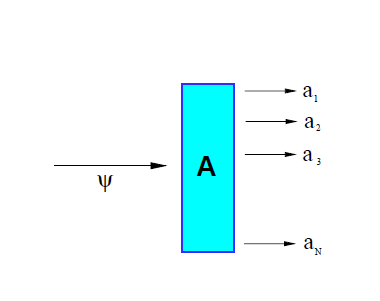
\includegraphics[width=10cm]{6_1.png}
\end{figure}

\section{تداخل}
حال به مهم‌ترین خصلت دنیای میکروسکوپی می‌رسیم. در شکل  درسمت چپ یک فیلامان حرارتی وجود دارد که بخاری از ذرات بار یونیزه را از خود متصاعد می‌کند.
 میدان‌های
الکتریکی به همراه مجموعه‌ای از یکسوکننده ها ذرات در حالت $\ket{P_{y}}$ را جدا می‌کنند. شکاف پایینی مسدود شده است.
 هر ذره
که از شکاف بالایی بگذرد درحالت $\ket{1}$ قرار می‌گیرد و سپس روی پرده در حالت ‏$\ket{y}$ که نقطه نشستن آن روی پرده را (توسط
یک آشکارساز) نشان می‌دهد، ثبت می‌شود.
 هرگاه این آزمایش را برای مدت طولانی انجام دهیم، در اثر نشستن ذرات روی
یک پرده - مثلا یک پرده فلورسانس - طرح $I_{1}$ بوجود خواهد آمد. 
$I_{1}(y)$ درواقع متناسب با تعداد ذرات نشسته شده روی نقطه $y$ است. درحقیقت داریم


\begin{equation}
	I_{1}(y) = P(y,1)P(1,P_{y})
\end{equation}

\begin{figure}[h]
	\caption{ آزمایش دو شکاف: تنها شکاف بالایی باز است و طرح $I_{1}$ روی پرده مشاهده می‌شود. }
	\centering
	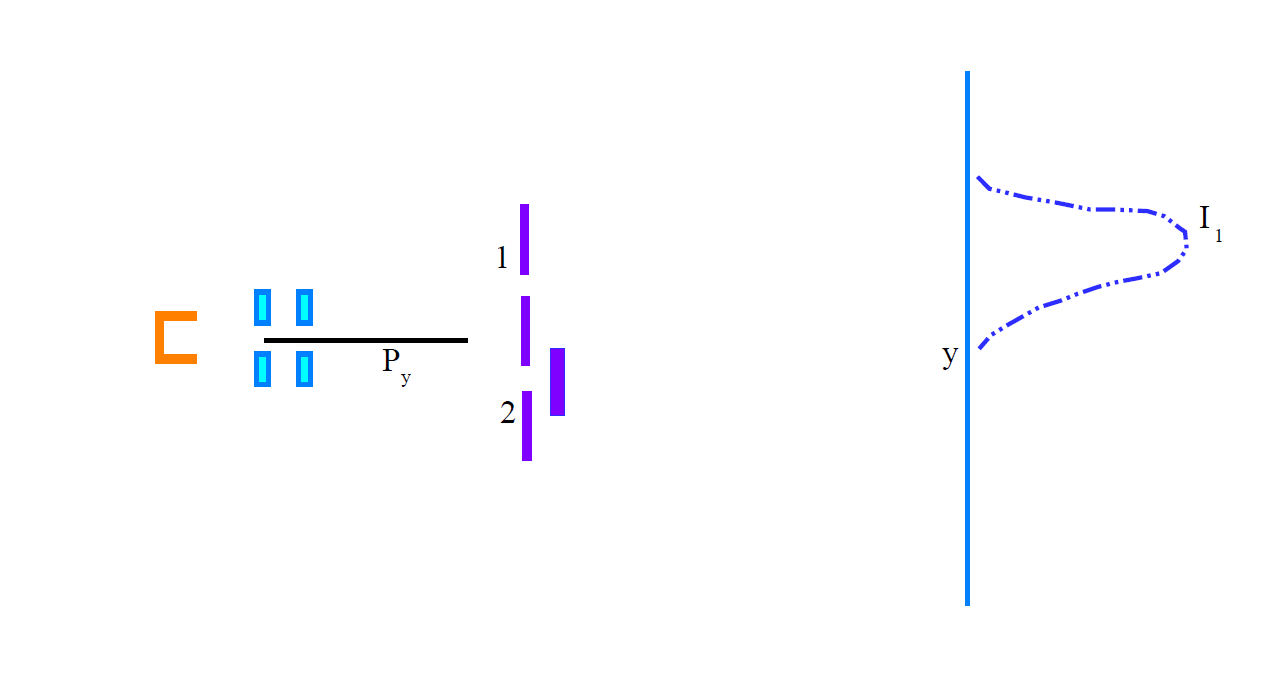
\includegraphics[width=10cm]{6_2.png}
\end{figure}
حال آزمایش را در حالتی که تنها شکاف پایینی باز باشد تکرار می‌کنیم. به همان معنا رابطه پیشین داریم: 
\begin{equation}
	I_{2} =  P(y,2)P(2,P_{y})
\end{equation}
\begin{figure}[h]
	\caption{ آزمایش دو شکاف: تنها شکاف پایینی باز است و طرح $I_{2}$ روی پرده مشاهده می‌شود. }
	\centering
	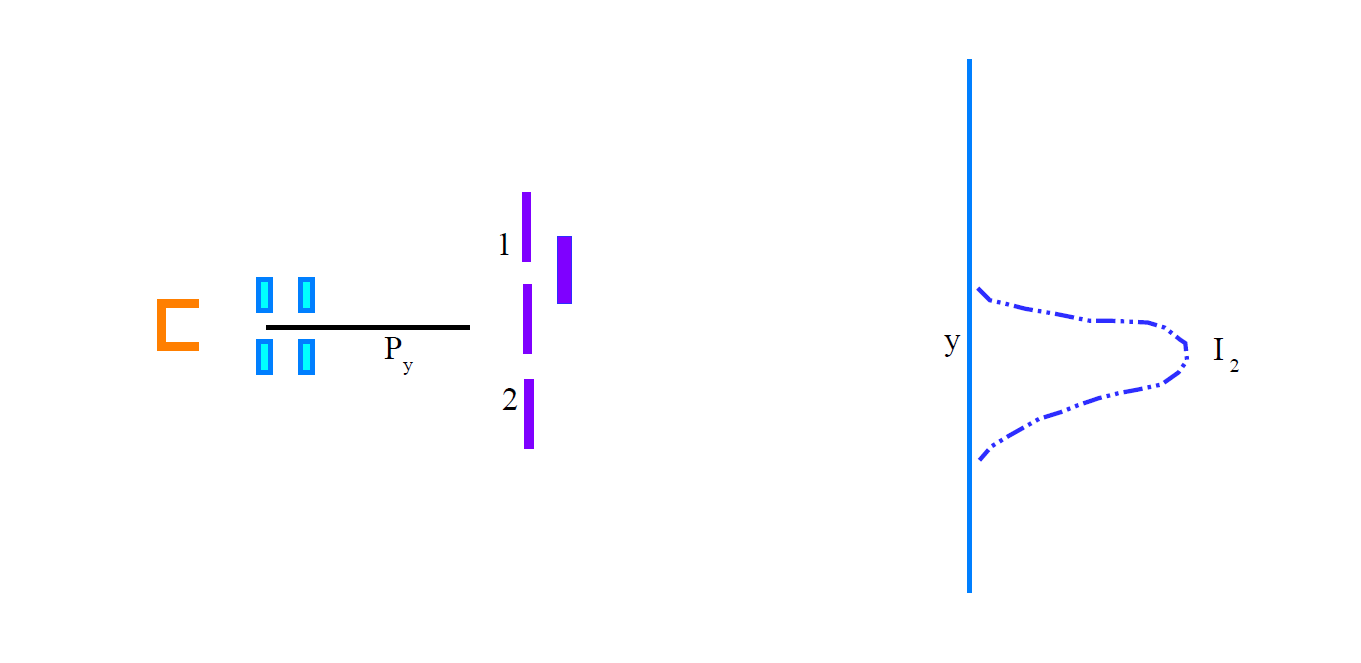
\includegraphics[width=10cm]{6_3.png}
\end{figure}
سپس آزمایش را در حالتی تکرار می‌کنیم که هر دو شکاف باز هستند. انتظار داریم این بار رابطه زیر برقرار باشد:

\begin{equation}
	I_{1 + 2} =  P(y,1)P(1,P_{y}) + P(y,2)P(2,P_{y}) = I_{1} + I_{2}
\end{equation}
و شکل \ref{fig:1} مشاهده شود.
\begin{figure}[h]
	\caption{ آزمایش دو شکاف: هر دو شکاف باز هستند و طرح $I_{1+ 2}$ روی پرده مورد انتظار است.  }
	\centering
	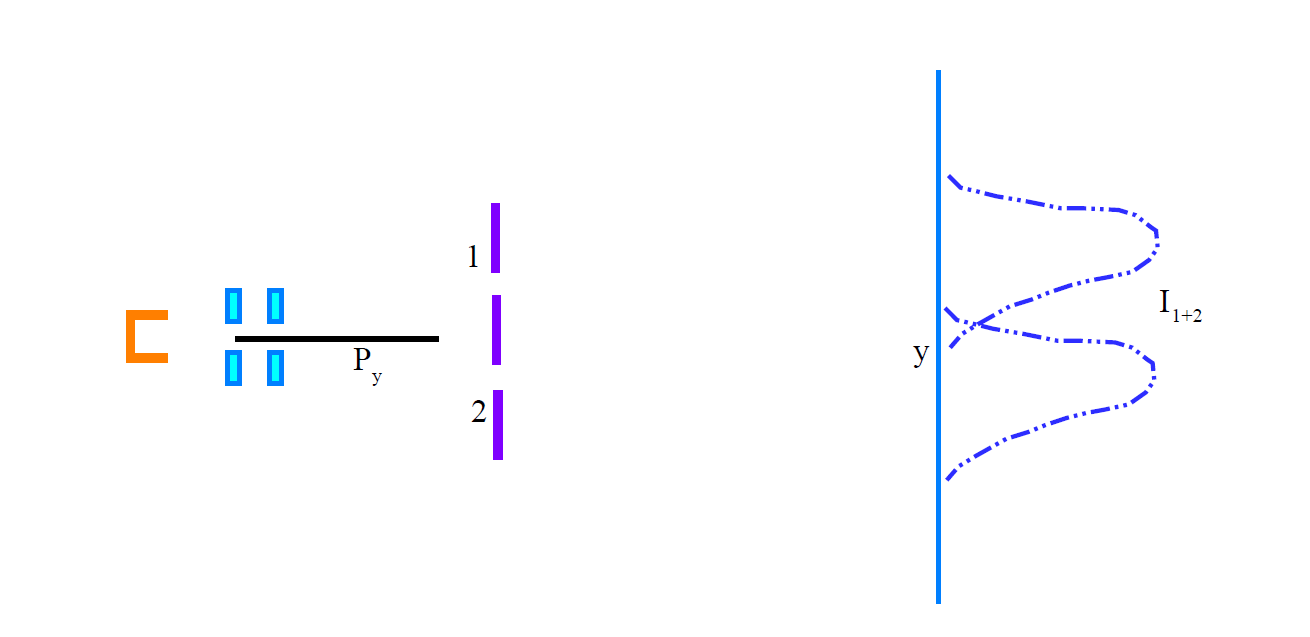
\includegraphics[width=10cm]{6_4.png}
	\label{fig:1}
\end{figure}

 


اما آنچه که در آزمایش می بینیم آن است که ذرات مطابق با طرح $I_{12}$ که یک طرح تداخلی است روی پرده می‌نشینند. (شکل \ref{fig:2})
\begin{figure}[h]
	\caption{ آزمایش دو شکاف: هر دو شکاف باز هستند و طرح $I_{1+ 2}$ روی پرده رخ می‌دهد.  }
	\centering
	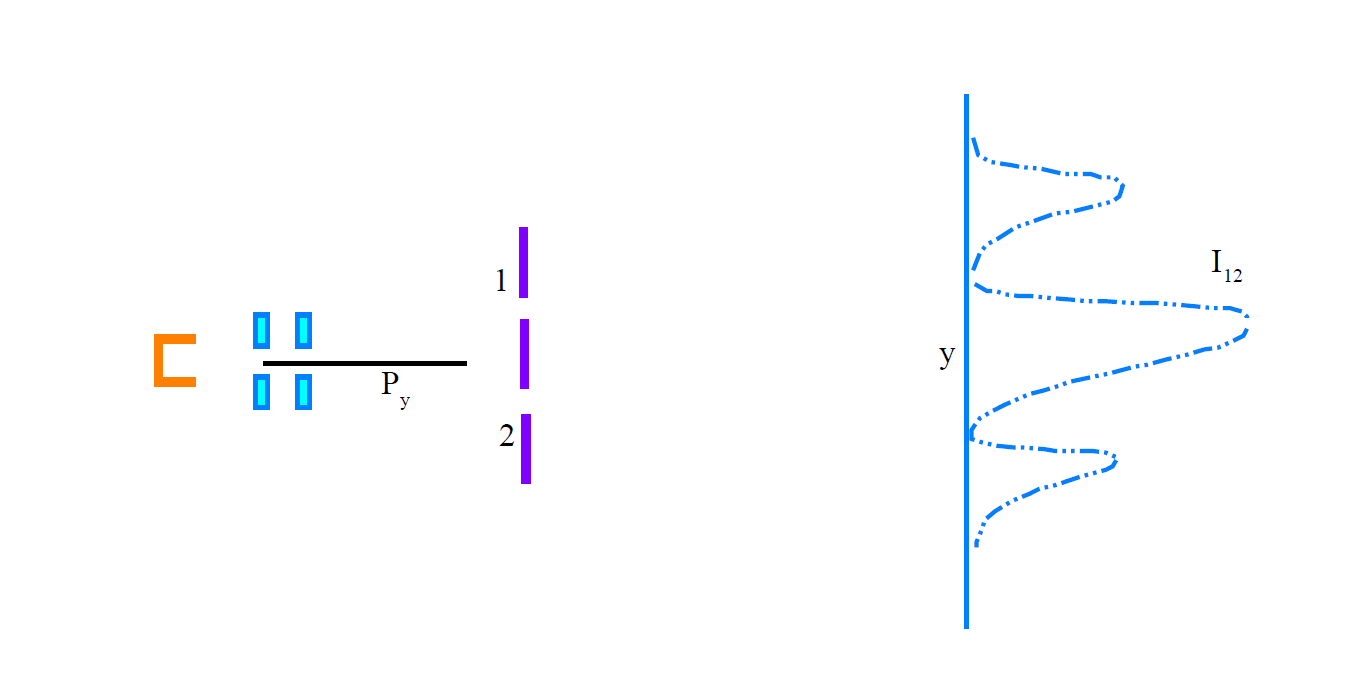
\includegraphics[width=10cm]{6_5.png}
	\label{fig:2}
\end{figure}

دراین طرح چندین نکته جالب و شگفت انگیز وجود دارد:

 

الف : در جاهایی از پرده، بازکردن هر دو شکاف با هم، باعث شده است که تعداد حتی کم‌تری ذرات نسبت به وقتی که تنها یک
شکاف بازبود به آن نقطه برسد. در جاهایی نیز مثل وسط پرده تعداد ذرات دو برابر آن مجموع تعداد ذراتی است که درصورت
باز بودن هرکدام از شکاف‌ها به تنهایی به پرده می‌رسید.

ب : برعکس درجاهای دیگری از ذرات باز کردن هر دو شکاف باعث شده است که تعداد ذراتی که به آن نقطه می‌رسد، بیشتر
از مجموع ذراتی شود که درصورتی که هر دو شکاف باز می‌بود به آن نقطه می‌رسید.

ج : شکل این طرح تداخلی با رقیق کردن چشمه ذرات بطوری که درهر آن فقط و فقط یکی از ذرات از شکاف ها عبور کند، تغییر نمی‌کند. بنابراین نمی‌توان گفت که ذرات هنگام باز بودن هر دو شکاف با یکدیگر طوری برهم‌کنش می‌کنند که اثرات بالا
دیده شود.

د : هرکدام از ذرات را روی پرده نهایی به طور کامل توسط آشکارساز ثبت می‌کنیم و آشکارساز ما ماهیت ذره‌ای آن را
به‌خوبی تایید می‌کند. بنابراین نمی‌توان گفت که ذره در این آزمایش مثل یک موجود پیوستار عمل کرده است و بخشی از آن از
یک شکاف و بخشی دیگراز یک شکاف دیگر عبور کرده است.

  
ه: ممکن است که ذره در حین عبور از دو شکاف به صورت یک پیوستار (چیزی شبیه
یک ابر) رفتار می‌کند و سپس در انتها موقع نشستن روی پرده تمامی این ابر دوباره به صورت یک ذره کوچک متمرکز می‌شود.
برای پی بردن به راز رفتار ذره می توان درست پشت شکاف ها آشکارسازهایی گذاشت تا بفهمیم که ذره درست موقع عبور از
شکاف‌ها چگونه رفتار می‌کند. متوجه می‌شویم که درآنجا هم ذره به صورت یک ابر رفتار نمی‌کند بلکه به تمامی (با تمام جرم و بار و دیگر خصوصیات خود) درآشکار ساز ثبت می‌شود. تلاش ما برای پی بردن به راز رفتار ذره باعث شده است که طرح تداخلی $I_{12}$
 از بین برود و جای خود را به طرح معمولی داده است. 
 
و :  منطق ساده به ما حکم می‌کند که هر ذره‌ای که
روی پرده می‌نشیند یا از شکاف ۱ آمده است یا از شکاف ۲. تعداد ذراتی که روی پرده نشسته‌اند برابرند با تعداد ذراتی که از
شکاف ۱ آمده اند + تعداد ذراتی که از شکاف ۲ آمده اند. اما تعداد ذراتی که از شکاف ۱ عبور کرده وروی پرده نشسته‌اند
برابراست با $I_{1}$ و تعداد ذراتی که از شکاف ۲ عبور کرده وروی پرده نشسته اند برابر است با $I_{2}$. پس حتی بدون مشاهده نزدیکی
شکاف‌ها می توانیم حکم کنیم که طرحی که سرانجام روی پرده ثبت می‌شود، می‌بایست برابر با $I_{1} + I_{2}$ باشد. درصورتی که اتم
ها مثل توپ فوتبال عمل کرده باشند استدلال بالا صحیح است. 
درمقابل ایراداتی ازاین نوع که « بالاخره الکترون یا ازاین شکاف عبور می‌کند ویا از آن شکاف و دراین صورت نمی‌بایست طرح تداخلی داشته باشیم» تنها می‌توانیم به این بسنده کنیم که بگوییم وقتی
سوال عبور الکترون از شکاف ها را به صورت عملی و تجربی بپرسیم می‌بنیم که طرح تداخلی واقعا از بین می‌رود
و ما به تناقضی برنمی‌خوریم. بنابراین می‌گوییم که وقتی الکترون را مشاهده نمی‌کنیم، نمی‌توانیم مسیری برای آن تعریف کنیم. 
 
 نخستین کار ما آن است که ببینیم آیا نظمی در طرح تداخلی شکل وجود دارد یا نه. به نظر می‌رسد که طرح $I_{12}$، یک طرح ناشی از تداخل امواج باشد. 
 بنابراین، برای پیداکردن نظمی که درجستجوی آن هستیم به تجربیات خود درمورد
امواج بازمی‌گردیم . اگر $I_{1}$ را مربع یک عدد مختلط $\phi_{1}$ موسوم به دامنه احتمال و $I_{2}$ را نیز مربع یک عدد مختلط $\phi_{2}$ بگیریم
چه بسا که $I_{12}$ مربع $\phi_{1} + \phi_{2}$ باشد، چنان که درمورد امواج چنین است:

 
\begin{equation}
	I_{1} := |\phi_{1}|^{2} \quad I_{2} := |\phi_{2}|^{2} \quad I_{12} =: |\phi_{12}|^{2}
\end{equation}
به طوری که 
\begin{equation}
	\phi_{12} = \phi_{1} + \phi_{2}
\end{equation}
و در معادله موج زیر، جملات سوم و چهارم که به جملات تداخلی موسوم هستند می‌توانند رفتار موجی ذرات را توجیه کنند:
 \begin{equation}
 	I_{12} = I_{1} + I_{2} + \phi_{1}\phi^{*}_{2} + \phi_{2}\phi^{*}_{1}
 \end{equation}
 
 ولی باید توضیح دهیم این اعداد مختلط چه هستند. فرایند تغییر حالت در این وضعیت، نباید به حالاتی که یک الکترون در میانه را طی می‌کند توجهی کند، پس متغیر $\phi_{12}$ دامنه احتمالی است که یک حالت اولیه را به یک حالت نهایی می‌برد:
  \begin{equation}
  	\phi_{12} = \braket{y}{P_{y}}
  \end{equation}
    \begin{equation}
  	\phi_{1} = \braket{y}{1}\braket{1}{P_{y}}
  \end{equation}
    \begin{equation}
  	\phi_{2} = \braket{y}{2}\braket{2}{P_{y}}
  \end{equation}
  توجه کنید که از نمادگذاری فوق منظوری از ضرب داخلی نداریم. در نتیجه:
   \begin{equation}
   		\braket{y}{P_{y}} = \braket{y}{1}\braket{1}{P_{y}} + \braket{y}{2}\braket{2}{P_{y}}
   \end{equation}
    این رابطه، اصل رابطه‌ای است که ساختمان نظری مکانیک کوانتومی بر اساس آن بیان می‌شود.
    \begin{equation}
    	\braket{c_{k}}{a_{i}} = \sum_{j} \braket{c_{k}}{b_{j}}\braket{b_{j}}{a_{i}}
    \end{equation}
    پس برای شکل مشخص است که می‌توانیم با آزمایش‌های مکرر، مقدار احتمال‌های زیر را حساب کنیم و داخل یک بردار به شکل زیر نشان دهیم:
    \begin{equation}
    	\ket{\Psi}_{A} = \begin{pmatrix}
    	\braket{a_{1}}{\Psi} \\ \\
    	\braket{a_{2}}{\Psi} \\ \\
    	\vdots \\ \\
    	\braket{a_{N}}{\Psi} \\ \\
    	\end{pmatrix}
    \end{equation}
    شاخص $A$ برای یادآوری آن است که اعداد داخل این بردار از اندازه‌گیری‌های $A$ به دست آمده است. 
    
   با توجه به قانون برابری احتمال 
   \begin{equation}
   P(a,b) = P(b,a) \longleftrightarrow \braket{a}{b} = \braket{b}{a}^{*}
   \end{equation}
   پس طبق رابطی کلی زیر 
   \begin{equation}
   	\braket{b_{j}}{\Psi} = \sum_{i} \braket{b_{j}}{a_{i}}\braket{a_{i}}{\Psi}
   \end{equation}
   می‌توان شاخص‌های اندازه‌گیری را حذف کرد و اطمینان دهیم که حالت ذره توسط بردار $\Psi$ توصیف شده است. با توجه به این که مقادیر بردار اندازه‌گیری احتمال هستند، ضرب‌کردن همه مقادیر در یک فاز، احتمالات را در یک شاخص اندازه‌گیری عوض نخواهد کرد. 
   
   \section{معادله شرودینگر}
   \begin{equation}
   	i\hbar \frac{\partial \psi}{\partial t} = H \psi
   \end{equation}
   معادله شرودینگر\footnote{Schrodinger Equation } نقش قوانین نیوتن در فیزیک کوانتوم را دارد. برای فهمیدن این معادله با فرمول بندی همیلتونی مکانیک کلاسیک\footnote{Hamiltonian Mechanics} شروع می‌کنیم. 
   \subsection{مکانیک همیلتونی}
   ذره‌ای با جرم $m$ را در نظر بگیرید که در یک فضای یک بعدی در حرکت است. مکان این ذره را با $q$ و تکانه\footnote{momentum} آن را با $p$ نمایش می‌دهیم و فرض می‌کنیم که ذره در پتانسیل $V = V (q, t)$ قرار دارد. در این صورت انرژی کل ذره برابر است با
   \begin{equation}
   	H = T + V
   \end{equation}
  که $T = \frac{p^{2}}{2m}$ انرژی جنبشی آن است. دو معادله زیر را در نظر بگیرید.
  \begin{equation}
  \begin{cases}
  \dot{q} = \frac{\partial H}{\partial p} & \\
  \dot{p} = - \frac{\partial H}{\partial q} & 
  \end{cases}
  \end{equation}
از آنجا که $V$ مستقل از $p$ است، داریم
\begin{equation}
	\frac{\partial H}{\partial p} = \frac{\partial T}{\partial p} = \frac{p}{m}
\end{equation}
و لذا معادله اول چیزی جز تعریف تکانه $p = m\dot{q}$ نیست. به طور مشابه از آنجا که $T$ مستقل از $q$ است از معادله دوم به دست می‌آوریم
\begin{equation}
	\dot{p} = - \frac{\partial V}{\partial q}.
\end{equation}
در نتیجه از ترکیب این دو داریم
 \begin{equation}
 	m\ddot{q} = - \frac{\partial V}{\partial q}
 \end{equation}
 که همان قانون دوم نیوتن است. در واقع معادله شرودینگر، فرمول بندی معادلی با $F = ma$ است که به آن فرمول بندی همیلتونی گفته می‌شود و کل مکانیک کلاسیک را می‌توان براساس آن پایه ریزی کرد.  
  \section{اصول مکانیک کوانتومی}
  \subsection{اصل اول - فضای حالات}
 به هر سیستم فیزیکی یک فضای هیلبرت متناظر است. حالت  سیستم (در هر لحظه از زمان)
با یک بردار ناصفر در فضای هیلبرت مشخص می‌شود. دو بردار که ضریبی از یکدیگر باشند یک حالت
فیزیکی را بیان می‌کنند. بنابراین حالت سیستم را می‌توان با یک بردار به طول یک (بردار واحد) مشخص
کرد.

فضای هیلبرت فضای برداری است که دارای ضرب داخلی باشد و نسبت به نرمی که ضرب داخلی آن القاء می‌کند، کامل باشد. توجه کنید که فضاهای ضرب داخلی با بعد متناهی همواره کامل هستند.

\begin{example}
کیوبیت یک سیستم کوانتومی است که فضای هیلبرت $H$ متناضر با آن دوبعدی باشد. اگر پایه تعامد یکه $\{\ket{0},\ket{1}\}$ را برای این فضا در نظر بگیریم، آن‌گاه داریم:
\begin{equation}
	\forall \ket{\Psi} \in H, \quad \ket{\Psi} = a\ket{0} + b\ket{1}, \quad a,b \in \mathbb{C}
\end{equation}   
\begin{equation}
	\| \ket{\Psi} \| = 1 \Rightarrow |a|^{2} + |b|^{2} = 1
\end{equation}   
بردار یکه $\frac{1}{\sqrt{2}}\ket{0} + \frac{1}{\sqrt{2}}\ket{1}$ مثالی از یک حالت است که یک کیوبیت می‌تواند داشته باشد. از آنجا که این بردار ضریبی از بردار یکه $-\frac{1}{\sqrt{2}}\ket{0} - \frac{1}{\sqrt{2}}\ket{1}$ است، این دو بردار یک حالت سیستم را نشان می‌دهند. تفاوت این دو بردار یکه ضریب کلی با نرم یک است و لذا به عنوان حالات کوانتومی، یکسان هستند. توجه کنید که این دو، با حالت $\frac{1}{\sqrt{2}}\ket{0} - \frac{1}{\sqrt{2}}\ket{1}$ متفاوت هستند چون ضریبی از یکدیگر نیستند.
\end{example}

 یک سیستم فیزیکی که بعد فضای هیلبرت متناظر آن $d$ باشد، $dim(H) = d$ یک کیودیت\footnote{Qudit} نامیده می‌شود. فضای برداری متناظر با یک کیودیت با پایه متعامد یکه زیر نمایش داده می‌شود:
  \begin{equation}
  \{ \ket{0}, \ket{1}, ... , \ket{d-1} \}
  \end{equation}
  
  \subsection{اصل دوم - تحول زمانی}
  تحول زمانی یک سیستم بسته با یک عملگر یکانی که روی فضای هیلبرت عمل می‌کند، بیان می‌شود. یعنی اگر حالت سیستم در زمان $t_{0}$، $\ket{\Psi}$ باشد و در زمان $t_{1}$، $\ket{\Psi^{'}}$ باشد، آنگاه $U \mathcal{H} \to \mathcal{H}$  یکانی وجود دارد که $U\ket{\Psi} = \ket{\Psi^{'}}$. $U$ تنها وابسته به زمان است. 
  
  این اصل در واقع فرمول بندی دیگری از اصل شرودینگر است. این معادله تحول زمانی یک سیستم کوانتومی را به صورت زیر بیان می‌کند: 
  \begin{equation}
  	i\hbar\frac{d}{dt}\ket{\Psi (t)} = H\ket{\Psi (t)}
  \end{equation}
  که در آن $H: \mathcal{H} \to \mathcal{H}$ یک عملگر هرمیتی است. اگر $H$ مستقل از زمان باشد،حل معادله دیفرانسیل فوق به صورت زیر است: 
  \begin{equation}
  	\ket{\Psi (t)} = \exp{-\frac{it}{\hbar}H}\ket{\Psi (0)}
  \end{equation}
  حال اگر قرار دهیم 
 \begin{equation}
 	U = \exp{-\frac{it}{\hbar}H}
 \end{equation}
 آنگاه معادله زمان اولیه برقرار می‌شود. می‌توان نشان داد $U$ یکانی است و این شرایط برای حالتی که $H$ مستقل از زمان هم نیست برقرار است. 
 
\begin{example}
  تحول زمانی یک کیوبیت با ماتریس‌های یکانی $2 \times 2$ مانند ماتریس‌های یکانی و هرمیتی زیر که آن‌ها را ماتریس پاولی\footnote{Pauli Matrices} می‌نامیم، بیان می‌شود: 
 \begin{equation}
 	X = \begin{pmatrix}
 		0 & 1 \\ \\
 		1 & 0 
 	\end{pmatrix}
 \end{equation}
 \begin{equation}
 	Z = \begin{pmatrix}
 		1 & 0 \\ \\
 		0 & -1 
 	\end{pmatrix}
 \end{equation}
 این عملگرها به صورت زیر عمل می‌کنند: 
 \begin{equation}
 	X(a\ket{0} + b\ket{1}) = a\ket{1} + b\ket{0}
 \end{equation}
  \begin{equation}
 	Z(a\ket{0} + b\ket{1}) = a\ket{0} - b\ket{1}
 \end{equation}
 \end{example}

 یک مثال دیگر، عملگر یکانی هادامارد\footnote{Hadamard Matrix} است: 
 \begin{equation}
 	H = \frac{1}{\sqrt{2}}\begin{pmatrix}
 		1 & 1 \\ \\
 		1 & -1 
 	\end{pmatrix}
 \end{equation}
 توجه کنید که $H$ هرمیتی هم است و داریم $H^{\dagger}XH = Z$ که نتیجه می‌دهد ویژه‌مقادیر $X$ و $Z$ یکسان است. ویژه‌بردارهای $Z$ به علت آن‌ که در پایه استاندارد قطری است برابر با $\{\ket{1}, \ket{0} \}$ است و ویژه‌بردارهای $X$ برابرند با 
 \begin{equation}
 	\{ \ket{+} := \frac{1}{2}(\ket{0} +\ket{1}), \ket{-} := \frac{1}{2}(\ket{0} - \ket{1})
 \end{equation}
 و خواهیم داشت $H\ket{0} = \ket{+}$ و $H\ket{1} = \ket{-}$.
 
  \subsection{اصل سوم - اندازه‌گیری}
اندازه گیری بر روی یک سیستم با فضای هیلبرت $\mathcal{H}$ با مجموعه‌ای به صورت 
\begin{equation}
	\{ M_{i}: M_{i}: \mathcal{H} \to \mathcal{H}, i \in S \}
\end{equation}
 مشخص می شود که :
 \begin{equation}
 	\sum_{i \in S} M_{i}^{\dagger}M_{i} = I 
 \end{equation}
 در این صورت به $M_{i}$ها عملگرهای اندازه‌گیری می‌گویند. با انجام این اندازه‌گیری، اگر حالت سیستم $\ket{\Psi} \in \mathcal{H}$ باشد، حاصل اندازه‌گیری با احتمال $p(i) = \ev{M_{i}^{\dagger}M_{i}{\Psi}}$ برابر می‌شود. اگر هم حاصل اندازه گیری $i$ باشد، حالت سیستم به 
 \begin{equation}
 	\ket{\Psi^{'}} = \frac{M_{i}\ket{\Psi}}{\sqrt{p(i)}}
\end{equation}  
تغییر\footnote{collapse} می‌کند.

\begin{example}
اندازه‌گیری یک کیوبیت، اگر $M_{i} = \dyad{v_{i}{v_i}}$ باشد، آنگاه می‌توان نشان داد که $\{ M_{0}, M_{1},...,M_{d-1}\}$ یک اندازه‌گیری است. 
پس اگر حالت سیستم به صورت $\ket{\Psi} = \sum_{i} a_{i}\ket{v_{i}}$ باشد، آنگاه
\begin{equation}
	p(i) = \ev{M_{i}^{\dagger}M_{i}}{\Psi} = |a_{i}|^{2}
\end{equation}
\end{example}

\begin{example}
اندازه‌گیری تصویری: عملگرهای تصویر را در نظر بگیرید. می‌توان نشان داد که $\{ P_{i}: i \in S \}$ یک اندازه‌گیری است. به چنین اندازه‌گیری تصویری می‌گویند. توجه کنید که در اندازه‌گیری تصویری، برای هر $i \ne j$ می‌توان نشان داد $P_{i}P_{j} = 0$. در واقع اگر تصویر $P_{i}$ را با $W_{i}$ نشان دهیم، آنگاه $\mathcal{H} = \bigoplus_{i \in S} W_{i}$ افراز فضا به زیرفضاهای عمود بر هم است. 
\end{example}

\begin{example}
یک مشاهده‌پذیر\footnote{Observable} فیزیکی با یک عملگر هرمیتی روی فضای هیلبرت مشخص می‌شود: 
\begin{equation}
A: \mathcal{H} \to \mathcal{H}
\end{equation}
مثلا، عملگر همیلتونی متناظر با مشاهده‌پذیر انرژی است. از آن‌جایی که $A$ هرمیتی است، در پایه‌های متعامد یکه، قطری می‌شود. در واقع، اگر $\lambda_{i} \in \mathbb{R}$ ویژه‌مقادیر $A$ باشند و $W_{i}$‌ها زیرفضاهای تولید شده توسط ویژه‌بردارهای متناظر با $\lambda_{i}$ باشند، و $P_{i}$ را عملگر تصویر عمود بر روی این زیرفضا بگیریم، آنگاه 
\begin{equation}
	A = \sum_{i}\lambda_{i}P_{i}
\end{equation}
و از آنجا که بردارهای ویژه $A$ کل $\mathcal{H}$ را می‌پوشانند، داریم $\sum_{i} P_{i}$. پس اندازه گیری $\{P_{i}\}$ را داریم. 

اگر حالت $\ket{\Psi}$ را با $\{P_{i}\}$ اندازه‌گیری کنیم و حاصل اندازه‌گیری $i$ باشد، آنگاه می‌گوییم مقدار مشاهده‌پذیر $A$ برابر با $\lambda_{i}$  است. در این صورت، امید ریاضی این مشاهده پذیر که با $\expval{A}$ نشان داده می‌شود برابر است با
\begin{equation}
	\expval{A} = \sum_{i} \lambda_{i} p(i)  = \sum_{i} \lambda_{i} \mel{\Psi}{P_{i}}{\Psi} = \mel{\Psi}{\sum_{i} \lambda_{i} P_{i}}{\Psi} = \mel{\Psi}{A}{\Psi}
\end{equation}
\end{example}

\subsection{اصل چهارم - سیستم های ترکیبی}
فضای هیلبرت متناظر با یک سیستم فیزیکی که متشکل از $n$ سیستم کوچک‌تر است از ضرب تانسوری فضاهای کوچک‌تر بدست می‌آِید. 

به عبارت دیگر، اگر فضای هیلبرت متناظر با سیستم$i$-م $\mathcal{H}_{i}$ باشد، فضای هیلبرت متناظر با کل $n$ سیستم برابر است با 
\begin{equation}
	\mathcal{H}_{1} \otimes \mathcal{H}_{2} \otimes ... \otimes \mathcal{H}_{n}.
\end{equation} 
اگر سیستم $i$-م در حالت $\ket{\Psi_{i}} \in \mathcal{H}_{i}$ باشد، کل سیستم در حالت 
\begin{equation}
	\Psi_{1} \otimes \Psi_{2} \otimes ... \otimes \Psi_{n}.
\end{equation}
است. 

\section{درهم‌تنیدگی\footnote{Entanglement}}
دو کیوبیت  $A$ و $B$ را در نظر بگیرید. $\mathcal{H}_{A}$ و $\mathcal{H}_{B}$ فضای هیلبرت معادل هر کدام از این کیوبیت‌ها با پایه‌های $\{ \ket{0}_{A}, \ket{1}_{A}\}$ و $\{ \ket{0}_{B}, \ket{1}_{B}\}$ نمایش داده می‌شود. طبق اصل چهارم، فضای هیلبرت متناظر با سیستم ترکیبی این دو کیوبیت برابر است با 
 \begin{equation}
 	\mathcal{H}_{AB} = \mathcal{H}_{A} \otimes \mathcal{B}
 \end{equation}
 که با پایه متعامد یکه 
 \begin{equation}
 	\{ \ket{0}_{A} \otimes \ket{0}_{B}, \ket{0}_{A} \otimes \ket{1}_{B}, \ket{1}_{A} \otimes \ket{0}_{B},\ket{1}_{A} \otimes \ket{1}_{B}\}
 \end{equation}
  مشخص می‌شود که برابر است با:
    \begin{equation}
 	\{ \ket{00}_{AB}, \ket{01}_{AB}, \ket{10}_{AB},\ket{11}_{AB}\}.
 \end{equation}
 هر $\ket{\psi}_{AB} \in \mathcal{H}_{AB}$ به صورت ترکیب خطی از چهار عضو مجموعه بالاست. اگر $\ket{\psi}_{AB}$ را $\ket{\psi}_{AB} = \ket{v}_{A} \otimes \ket{w}_{B}$ نمایش داد به این حالت، حالت ضربی\footnote{Product State } و یا حالت جداپذیر\footnote{Seperable State} گفته می‌شود. اگر چنین نمایشی برای $\ket{\psi}_{AB}$ وجود نداشته باشد، به آن حالت درهم‌تنیده\footnote{Entangled State} می‌گویند. 
 \textbf{مثال: }
 \begin{equation}
 	\frac{1}{\sqrt{2}}(\ket{00} + \ket{01}) = \frac{1}{\sqrt{2}} \ket{0}_{A} \otimes (\ket{0}_{B} + \ket{1}_{B})
 \end{equation}
 یک حالت ضربی است و 
 \begin{equation}
 	\frac{1}{\sqrt{2}}(\ket{00} + \ket{11})
 \end{equation}
  یک حالت درهم‌تنیده‌است. 
  \section{اختتامیه‌ای بر عجایب مکانیک کوانتومی}
 کنترل اتم‌های منفرد و به همراه آن گسترش رایانش و اطلاعات کوانتومی منجر به پیدایش سوال‌های جدید در ساختمان نظری مکانیک کوانتومی
شده‌است. تلاش برای پاسخ‌گویی به این سوال‌ها به نوبه خود منجر به غنی شدن نظریه مکانیک کوانتومی از جهات متعدد شده است. به عنوان مثال،
چگونه می‌توان درهم‌تنیدگی دو حالت مثل 
\begin{equation}
	| \phi \rangle = \sqrt{0.9}|0,0\rangle + \sqrt{0.1}|1,1\rangle
\end{equation}
و 
\begin{equation}
	| \phi \rangle = \sqrt{0.8}|0,0\rangle + \sqrt{0.2}|1,1\rangle
\end{equation}
را با هم مقایسه کرد؟
مثل هر ویژگی دیگری در فیزیک باید بتوانیم به صورت کمی مقدار درهم‌تنیدگی این دو حالت را با هم مقایسه کنیم.

چگونه می‌توان بیشتر از دو ذره را در هم تنیده کرد؟ اکنون می‌توانیم جفت فوتون هایی را که بیش از یکصد و پنجاه کیلومتر از یکدیگر دور هستند، در‌هم‌تنیده کنیم. سوال این است که چگونه
می‌توانیم با انجام آزمایش در هرکدام از آزمایشگاه‌ها مقدار این درهم‌تنیدگی را کم و زیاد کنیم. 
چگونه می‌توانیم این کار را برای جفت فوتون‌هایی که بین زمین و ماهواره ها درهم تنیده هستند انجام دهیم؟ چگونه می توانیم اتم‌های ساکن دور از هم را درهم تنیده کنیم؟ آیا می‌توانیم شبکه‌ای از حالت های درهم تنیده بین نقاط مختلف و دور از هم درست کنیم و از آن برای مبادله اطلاعات کوانتومی و فرابرد کوانتومی استفاده کنیم؟

سوالات در مورد درهم تنیدگی نه تنها از نظر عملی مهم هستند بلکه از نظر ریاضی نیز اهمیت دارند. ما شناخت نسبتا کاملی از فضای هیلبرت
دو کیوبیت داریم. مثلا می‌دانیم که حالتی مثل
\begin{equation}
	| \phi \rangle = \sqrt{0.5}|0,0\rangle + \sqrt{0.5}|1,1\rangle
\end{equation}
بیشترین میزان درهم تنیدگی را دارد و تمام حالت های دیگر را با اعمال موضعی می توان از این حالت درست کرد. در واقع می توانیم با سنجش
درهم‌تنیدگی تمام بردارهای فضای هیلبرت، دو ذره را مرتب کنیم. ولی به محض اینکه به فضای هیلبرت سه کیوبیت می رسیم با انواع سوال‌های
جدید و بی پاسخ مواجه می‌شویم و این وضعیت ساده از بین می رود. هیچ ملاک مقایسه‌ای نداریم که بر مبنای آن بگوییم کدام یک از دو حالت
\begin{equation}
	| GHZ \rangle = \sqrt{0.5}|0,0,0\rangle + \sqrt{0.5}|1,1,1\rangle
\end{equation}
یا 
\begin{equation}
	| W \rangle = \sqrt{1/3}(|1,0,0\rangle + |0,1,0\rangle +  |0,0,1\rangle )
\end{equation}
در هم تنیدگی بیشتری دارند. این گونه مطالعات به ما کمک می‌کنند که ملاک‌های معینی برای دسته بندی حالت‌های فضای هیلبرت دو و چند
ذره‌ای ابداع کنیم و بتوانیم فضای بسیار بزرگ هیلبرت را برای یک سیستم چند ذره‌ای بر اساس این خاصیت‌ها شناسایی کنیم. سوال‌ها و کشفیات
جدید البته منحصر به در هم تنیدگی نیستند و حوزه‌های خیلی وسیعی را در بر می‌گیرند. در ادامه به یک نوع دیگر از این سوال‌ها می‌پردازیم.
\section{قضایای عدم امکان در مکانیک کوانتومی}
در سال‌های اخیر و بعد از توجه دوباره به مبانی مکانیک کوانتومی، معلوم شده است که بعضی اعمال را در دنیای میکروسکوپی هرگز نمی‌توان
انجام داد. این قضایای عدم امکان\footnote{No go theorems} اهمیت نظری و عملی بسیار زیادی دارند. به عنوان مثال قضیه عدم تکثیر\footnote{No Cloning Theorem} که یک قضیه بسیار ساده
ولی مهم و بنیادی در مکانیک کوانتومی است ، تنها در سال 1982 یعنی هشتاد سال بعد از پیدایش مکانیک کوانتومی کشف شد . در زیر، یکی
از این قضایای عدم امکان را، که همگی به تازگی کشف شده‌اند، بیان می‌کنیم.
\subsection{تکثیر حالت‌های کوانتومی}
نخست ساده ترین حالت رادر نظر می‌گیریم. حالتی که می‌خواهیم آن راتکثیر کنیم با $|\phi\rangle$ نشان می‌دهیم. حالتی را که می خواهیم یک نسخه از $|\phi\rangle$ روی آن نوشته شود را با $|b\rangle$ نشان می‌دهیم. این حالت حکم کاغذ سفید را دارد و به همین دلیل آن را حالت سفید یا حالت خالی می‌نامیم. حالت  دستگاه را نیز با $|m\rangle$ نشان می دهیم. فرض کنید که یک عمل یکانی وجود دارد که برای هرحالت ورودی کار زیر را انجام می‌دهد: 
\begin{equation}
	U(|\phi\rangle\otimes|b\rangle\otimes|m\rangle) = |\phi\rangle \otimes |\phi\rangle \otimes |m_{\phi}\rangle)
\end{equation}
دراین صورت این دستگاه حالت یک نسخه از حالت ورودی را روی حالت سفید می‌نویسد و حالت خود دستگاه نیز بسته به حالت ورودی تغییر می‌کند. درخروجی دو نسخه از حالت $|\phi\rangle$ داریم. حال دو حالت متعامد $|0\rangle$ و $|1\rangle$ را در نظر می‌گیریم. حالت‌ زیر را هم در نظر بگیرید:
\begin{equation}
	|+\rangle = \frac{1}{\sqrt{2}} (|1\rangle + |0\rangle)
\end{equation}
حال، سه حالت $|0\rangle$ و $|1\rangle$ و $|+\rangle$ را به داخل ماشین تکثیر می‌فرستیم. دقت کنید که این دوحالت لزوماً دو حالت از یک سیستم دوبعدی نیستند. دراین صورت خواهیم داشت: 
\begin{equation}
	U(|0\rangle\otimes|b\rangle\otimes|m\rangle) = |0\rangle \otimes |0\rangle \otimes |m_{0}\rangle
\end{equation}
و 
\begin{equation}
	U(|1\rangle\otimes|b\rangle\otimes|m\rangle) = |1\rangle \otimes |1\rangle \otimes |m_{1}\rangle
\end{equation}
و
\begin{equation}
	U(|+\rangle\otimes|b\rangle\otimes|m\rangle) = |+\rangle \otimes |+\rangle \otimes |m_{+}\rangle
\end{equation}
اماهرگاه تساوی سوم را بسط دهیم و ازدو رابطه اول و خطی بودن مکانیک کوانتومی استفاده کنیم به رابطه زیر می‌رسیم:
\begin{equation}
|0\rangle|0\rangle|m_{0}\rangle + |1\rangle|1\rangle|m_{1}\rangle = 
\frac{1}{\sqrt{2}}(|0\rangle|0\rangle + |0\rangle|1\rangle + 
					|1\rangle|0\rangle + |1\rangle|1\rangle)|m_{+}\rangle
\end{equation}
هرگاه طرفین این رابطه را یک‌بار در $\langle 0|\langle 0|$ و یک‌بار در $\langle 1|\langle 1|$ ضرب کنیم، با استفاده از خاصیت متعامد بودن $|0\rangle$ و $|1\rangle$ به نتیجه زیر می‌رسیم:
\begin{equation}
	|m_{+}\rangle = \sqrt{2}|m_{0}\rangle = \sqrt{2}m_{1}\rangle
\end{equation}  
با جایگذاری این رابطه در رابطه قبلی و مقایسه دوطرف می‌رسیم به
\begin{equation}
	|0\rangle|1\rangle + |1\rangle|0\rangle = 0
\end{equation}
هرگاه طرفین این رابطه را در $\langle 0|\langle 1|$ ضرب کنیم به رابطه $1 = 0$ می‌رسیم که تناقض است. 

